\chapter{Docker Monitor}
\label{app:dockermonitor}
The script, Docker-stats.py is a Python-based graphical Docker container and process monitor. It connects to the Docker Engine on your computer, displays running containers and their resource usage, lets you inspect the processes inside each container, and provides a live log viewer.
It uses Tkinter for the graphical interface and the Python docker library to communicate with Docker.
The main features are:
\begin{itemize}
    \item Container monitoring - Lists running Docker containers, showing their names, abbreviated IDs, status, uptime, CPU usage, memory usage, network traffic, and exposed port mappings.
    \item Live resource statistics - Refreshes container discovery and resource statistics approximately every two seconds, displaying CPU utilization, memory consumption, and cumulative network bytes received and transmitted.
    \item Container process inspection - Expand a container in the interface to retrieve its process list using Docker's top() method. Individual processes are displayed as child rows with their command, PID, CPU percentage, and memory percentage.
    \item Live log viewer - Double-click a container or right-click and choose View Logs to open a separate log window. It initially loads the last 200 log entries, includes timestamps, continuously streams new entries, and automatically scrolls to the bottom.
\end{itemize}

\begin{figure}[H]
	\centering
		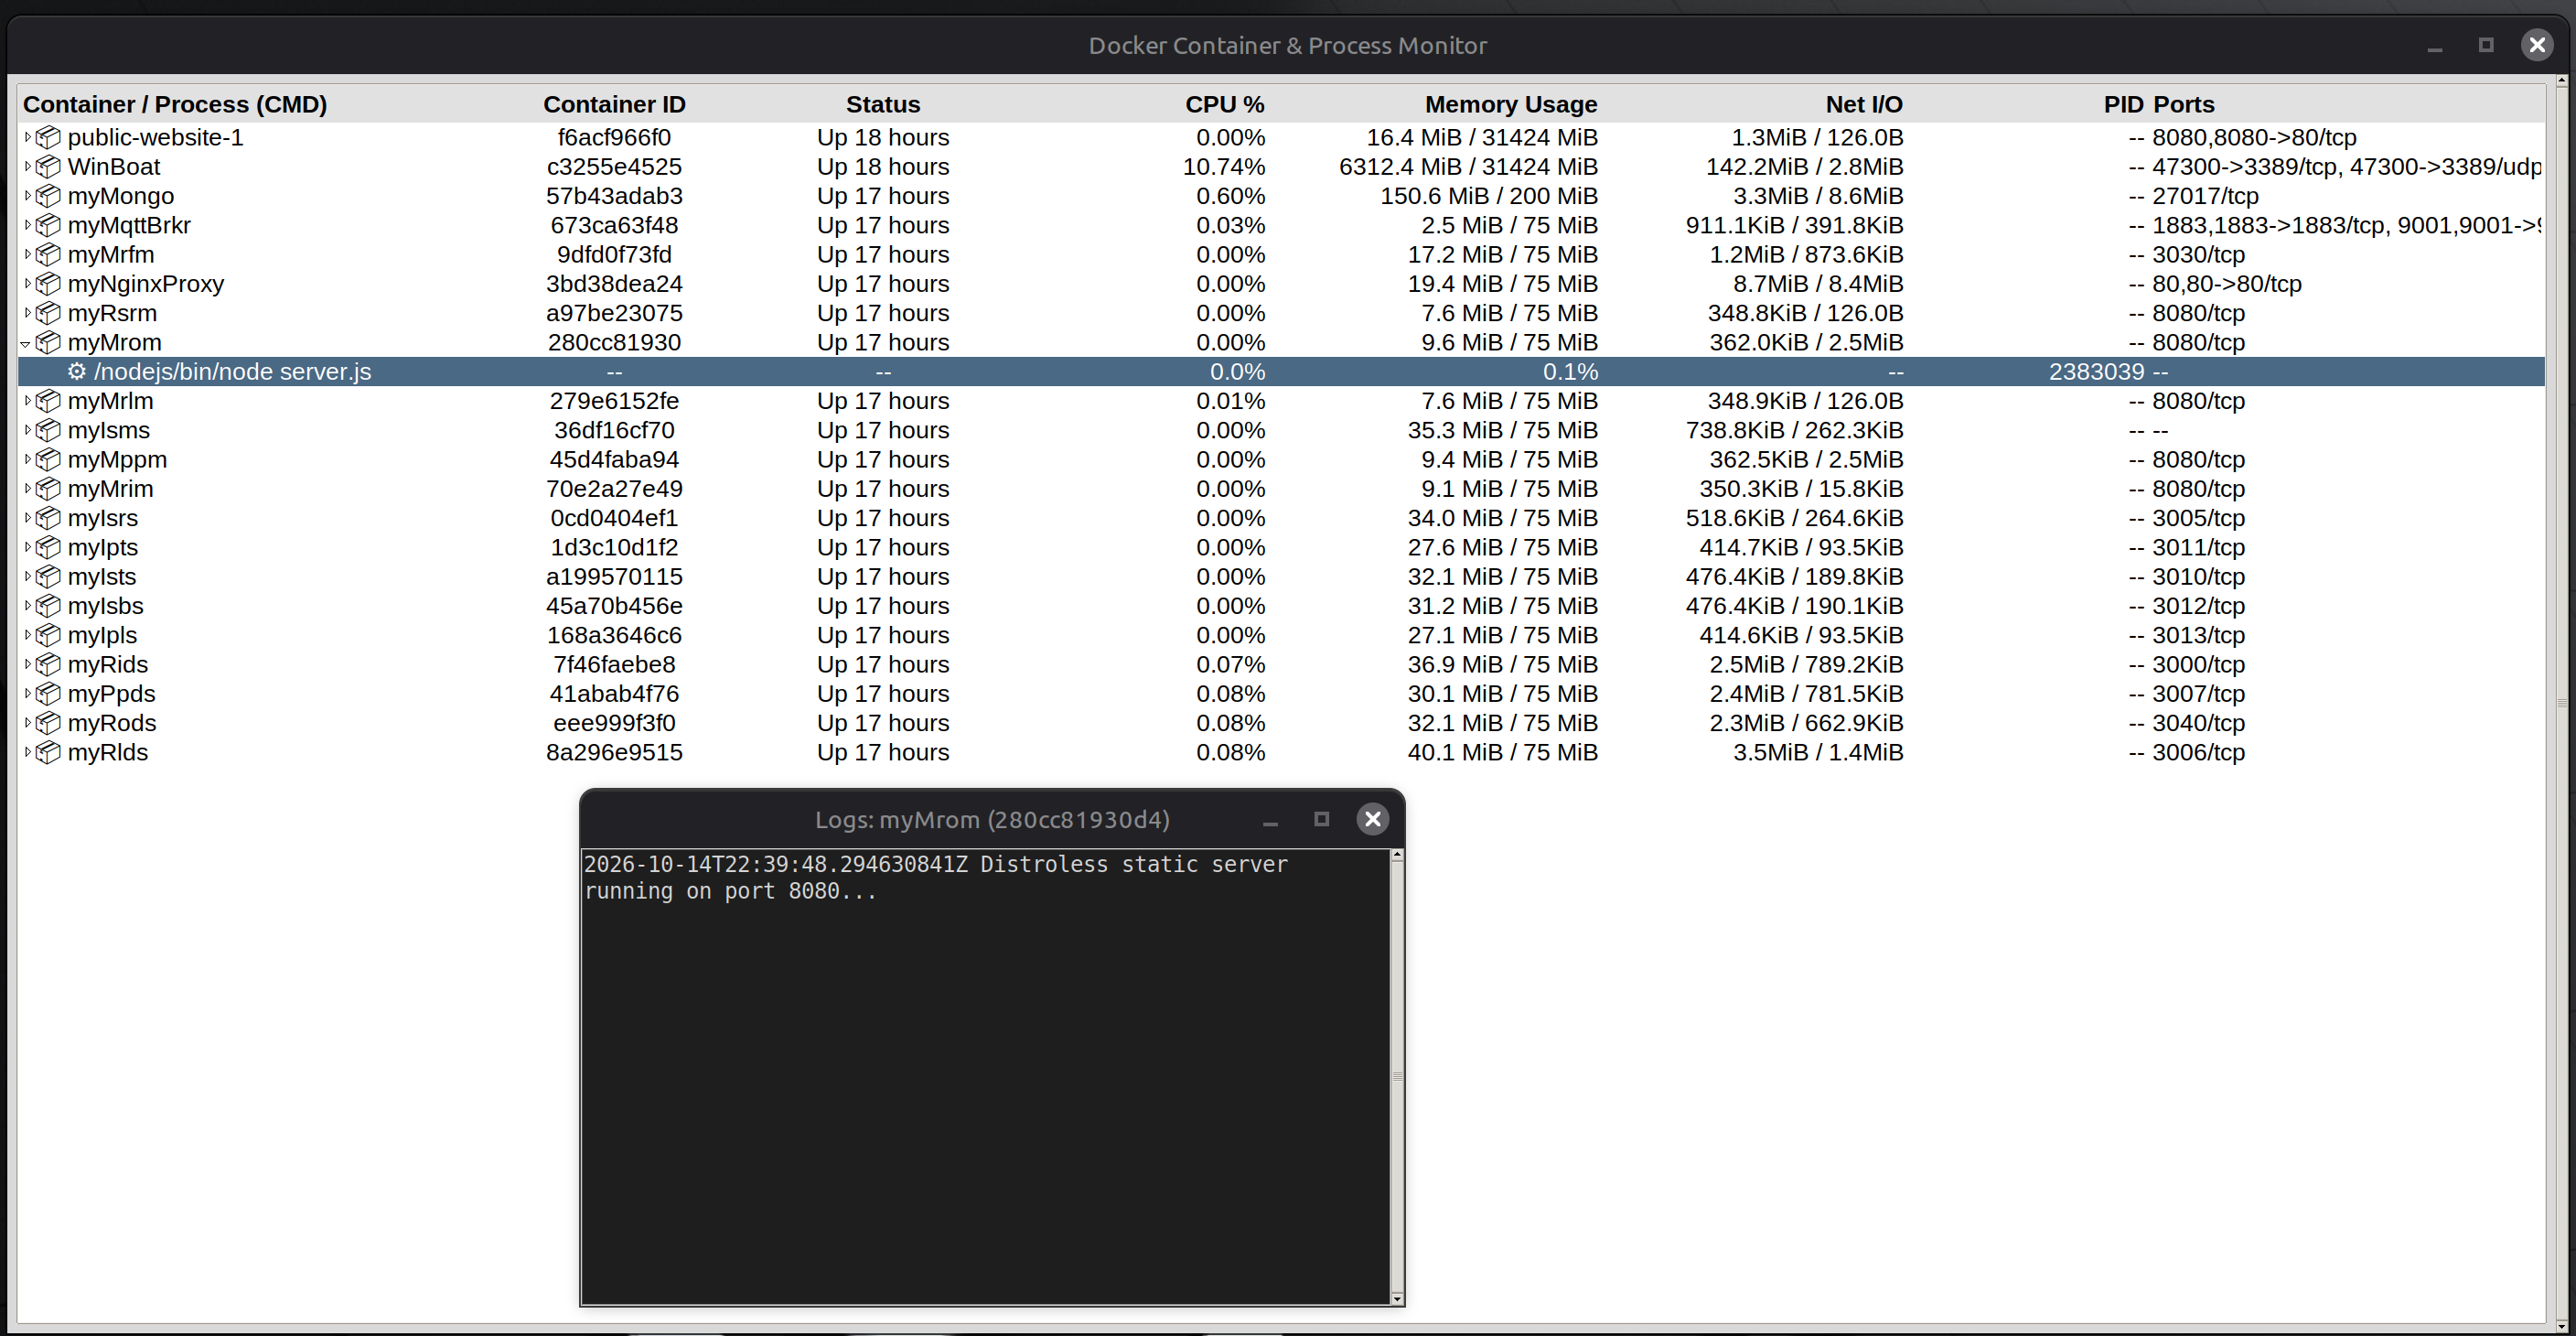
\includegraphics[scale=0.12]{../Images/docker-monitor.png}
	\caption{Docker Monitor}
	\label{fig:docker-monitor}
\end{figure}

To start the monitoring from a terminal enter the command:
\begin{verbatim}
python3 Docker-stats.py&
\end{verbatim}
The resulting window is shown in figure \ref{fig:docker-monitor}, it also depicts a window display a log of a container.
